\newpage
\section{Revisão da Teoria}

\subsection{Circuitos Ressonantes}

Os circuitos ressonantes podem se dispor de duas maneiras, em série ou em 
paralelo com elementos reativos como capacitor e indutor (figura \ref{fig:01}). 
São comumente 
utilizados em circuitos de banda estreita com aplicações em osciladores de 
baixo ruído.

\begin{figure}[H]
  \centering
  \caption{Circuito ressonante a) série b) paralelo.}
  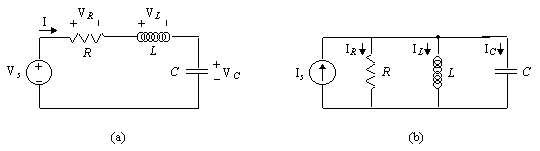
\includegraphics[scale=1]{01}
  
  \label{fig:01}
\end{figure}

A frequência de ressonância do circuito pode ser encontrada a partir dos 
elementos que o compõe. Para o circuito LC paralelo simples a frequência de 
ressonância é definida pela equação \ref{equ:f0}

\begin{equation}
  \label{equ:f0}
 f_0 = \frac{1}{2 \pi \sqrt{LC}}
\end{equation}

\subsection{Filtros Passivos}

Os filtros são circuitos que oferecem uma resposta em frequência com valores 
significativos em determinadas faixas.  Essas faixas são limitadas de acordo 
com os elementos do circuito e seus respectivos valores.
Os filtros passivos não amplificam o sinal de entrada, apenas selecionam 
frequências. A figura \ref{fig:02} apresenta algumas representações dos 
diversos tipos de filtros.

\begin{figure}[H]
  \centering
  \caption{ FPB, FPA, FPF e FRF.}
  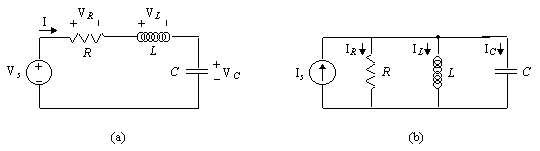
\includegraphics[scale=1]{01}
  
  \label{fig:02}
\end{figure}


\subsubsection{Filtros Passa-Baixas Passivo}

O filtro passa-baixas limita a frequência do sinal de saída entre zero e uma 
certa frequência de corte, atenuando frequências acima desta. Esse filtro pode 
ser arranjado de diferentes maneiras e com quantidades diferentes de elementos.
A figura \ref{fig:03} mostra alguns filtros passa-baixas passivos.

\begin{figure}[H]
  \centering
  \caption{Filtro Passa-Baixas, 1ª ordem, 2ª ordem e 3ª ordem.}
  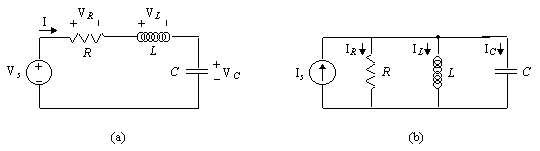
\includegraphics[scale=1]{01}
  
  \label{fig:03}
\end{figure}

\subsubsection{Filtros Passa-Alta Passivo}

O filtro passa-altas ajusta a frequência do sinal de saída para estar acima da 
frequência de corte, atenuando frequências abaixo desta. \cite{Stallings}.

\subsection{Fator de Qualidade}

O fator de qualidade é a razão entre a energia armazenada e a energia dissipada 
em R. Esse dado indica o desempenho do circuito e pode ser encontrado pela 
seguinte equação:

\begin{equation}
  \label{equ:Q}
  Q_{Load} = \frac{f_0}{BW_{3DB}}
\end{equation}

\subsection{Curva de Lissajous}

A curva de Lissajous é um gráfico obtido a partir de um sistema de equações 
paramétricas que descreve um comportamento harmônico. É muito utilizada para 
analisar a defasagem dada por dois sinais.
Para que a defasagem entre dois sinais possa ser obtida, os valores máximo e 
mínimo da curva devem ser observados, a distancia entre esses dois pontos 
representará o parâmetro A, bem como os valores de cruzamento com o eixo y, 
positivo e negativo, devem ser encontrados, e sua distância representará o 
parâmetro B. Com esses parâmetros, a defasagem poderá ser obtida através da 
seguinte equação:

\begin{equation}
\label{equ:lissa}
\Delta \Theta = sen^{-1}\left(\frac{B}{A}\right)
\end{equation}
